\section{Durchführung}
\label{sec:Durchführung}

Für alle Folgenden Messungen ist der Versuchsaufbau bis aus kleine Änderungen gleich.
Es wird auf einer optischen Bank eine Halogenlampe montiert.
Vor diese Lampe wird eine lichtundurchlässige Platte gestellt in der lichtdurchlässige Perlen in Form von einem L angeordnet sind.
Dieses Objekt wird von nun an als Perl-L bezeichnet.
Die Position des Perl-L's wird fixiert und notiert.
Als nächstes wird eine Linse und ein Schirm auf die optische Bank gestellt.

\subsection{Messung der Bildweite in Abhängigkeit der Gegenstandsweite}
\label{ssec:Durchführung_brennweite}

Eine Sammellinse mit bekannter Brennweite wird an einer bestimmten Gegenstandsweite fixiert und notiert.
Nun wird der Schirm so lange verschoben bis das Perl-L scharf auf dem Schirm abgebildet wird.
Die Bildweite wird notiert.
Diese Messung wird für 10 verschiedene Gegenstandsweiten und für zwei Linsen durchgeführt.
Die hier benutzten Linsen haben laut dem Hersteller eine Brennweite von $\SI{50}{\milli\metre}$ und $\SI{100}{\milli\metre}$.

\subsection{Messung der Brennweite nach der Methode von Bessel}
\label{ssec:Durchführung_bessel}

Auch für diese Messung wird eine Sammellinse mit vorgegebener Brennweite von $\SI{100}{\milli\metre}$ benutzt.
Der Schirm wird an einem festgelegten Abstand zum Perl-L fixiert.
Nun werden zwei Positionen für die Sammellinse gesucht, an denen die Abbildung des Perl-L scharf ist.
Die Gegenstandsweiten dieser Positionen werden notiert.
Die Messung wird für 10 verschiedene Schirmpositionen durchgeführt.

\begin{figure}
    \centering
    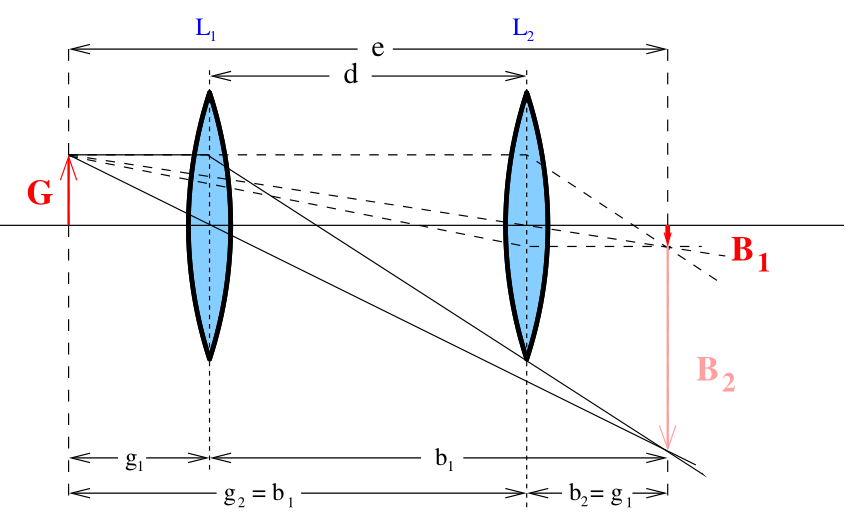
\includegraphics[width=0.5\textwidth]{images/skizze_bessel.png}
    \caption{Skizze der Methode von Bessel mit den zwei Linsenpositionen.\cite{V408}}
    \label{fig:skizze_bessel}
\end{figure}

\subsection{Messung der Brennweite eines Zusammengesetzten Linsensystems nach der Methode von Abbe}
\label{ssec:Durchführung_abbe}

Für die Messung nach der Methode von Abbe wird zunächst die Größe des Perl-L gemessen.
Dann wird eine Sammellinse und eine Zerstreuungslinse mit angegebener Brennweite von $\SI{\pm 100}{\milli\metre}$ auf der optischen Bank montiert.
Der Abstand der Linsen wird für die folgenden Messungen konstant gehalten und es wird ein Referenzpunkt $A$ gesucht, an dem der Abstand des Linsensystems zum Perl-L und zum Schirm abgemessen werden kann. (vgl. \autoref{fig:skizze_abbe})

\begin{figure}
    \centering
    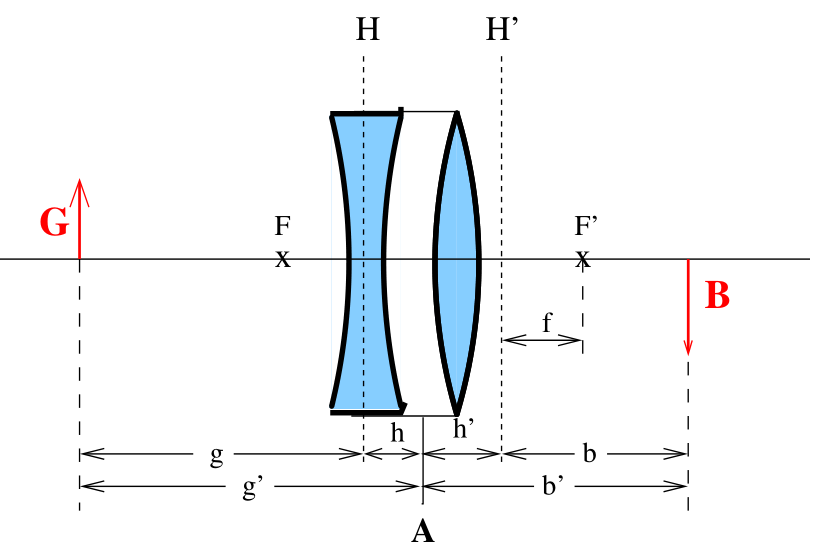
\includegraphics[width=0.5\textwidth]{images/skizze_abbe.png}
    \caption{Skizze der Methode von Abbe mit einem Linsensystem bestehend aus einer Zerstreuungs- und einer Sammellinse. \cite{V408}}
    \label{fig:skizze_abbe}
\end{figure}

Nun wird für 10 Verschiedene Abstände $g'$ der Schirm so verschoben, dass das Perl-L scharf abgebildet wird.
Der Abstand $b'$ wird gemessen und notiert.
Außerdem wird die Größe der Abbildung auf dem Schirm gemessen und notiert.

